
\chapter{\IfLanguageName{dutch}{Maatregelen voor ANPR}{Implementation guide for ANPR}}
\label{ch:maatregelenanpr}

In deze sectie beoordelen we welke maatregelen genomen moeten worden bij het implementeren van een ANPR systeem met oog op de parking aan de UGent.

Nummerplaatdetectie is al sterk geevolueerd sinds vroeger, maar heeft nog steeds enkele drawbacks. Zo spelen factoren zoals weer, belichting en plaatsing van de camera's een invloed op de nauwkeurigheid van de uitlezingen. Indien we met beperkte hardware werken kunnen deze omstandigheden niet altijd gemakkelijk direct verholpen worden, maar is het de bedoeling dat toch een optimale instelling behaald wordt.

\section{Cameraplaatsing}

\subsection{Locatie van de camera}
Uit een prototype van \textcite{arrieta2019prototype} bleek dat nummerplaten niet correct geïdentificeerd werden bij een inclinatiehoek vanaf 30 graden. Het is dus aanbevolen om de camerahoek te beperken tot een kleine hoek.

Verder is het aangeraden om de camera hoger te plaatsen dan de koplampen van de auto, dit om te voorkomen dat de camera verblind wordt door het sterke licht.

\subsection{Camera oriëntatie}
De gedetecteerde nummerplaten horen parallel te staan met de randen van de afbeelding. Dit omdat de datasets voor OpenANPR getraint zijn met afbeeldingen van horizontale nummerplaten, maar niet van gedraaide. Indien het niet mogelijk is om een rechte afbeelding te nemen kan de afbeelding ook later gedraaid worden.

\subsection{Pixeldichtheid}
Het aantal pixels van de foto waaruit een nummerplaat bestaat is van belang voor OpenALPR voor een duidelijke herkenning. Indien een foto van veraf is genomen zal deze laag zijn en van dichtbij zal deze dan weer hoog zijn. OpenALPR verwacht voor Europeaanse nummerplaten minstens een wijdte van 75 pixels en een grootte meer dan 250 pixels verhoogt niet opmerkelijk de accuraatheid. \autocite{openalprcameraplacement}

\section{Camera instellingen}
De belangrijkste factor van een performant ANPR-systeem is een correct ingestelde camera. Het nemen van foto's is de eerste stap in het proces en indien hierop nummerplaten niet duidelijk zijn kan OpenALPR onmogelijk iets detecteren. In dit onderdeel worden de belangrijkste instellingen verduidelijkt die bijdragen tot een correcte foto voor gebruik bij nummerplaatdetectie.

\subsection{Shuttersnelheid}
%\textcite{guo2017vehicle} stelt een trainingsmodel voor dat rekening houdt met blur.

Camera shutterspeed is de snelheid dat een camera foto's neemt. In een klaarlichte dag kan de shutterspeed zo'n 1/10000 seconden halen terwijl in het donker dit wel een volle seconde kan duren om genoeg licht te behalen. \autocite{openalprcameraplacement}

Bij een lange shutterspeed kan het dus zijn dat een voertuig een meter vooruit is gereden, terwijl bij een kleine shutterspeed dit bv. maar een centimeter is. Een korte shutterspeed is dus interessant voor het implementeren van nummerplaatdetectie aangezien de auto minder ver is gereden en dus minder motion blur op de foto staat.
%
\begin{figure}[h!]
	\centering
	\begin{subfigure}[b]{0.4\linewidth}
		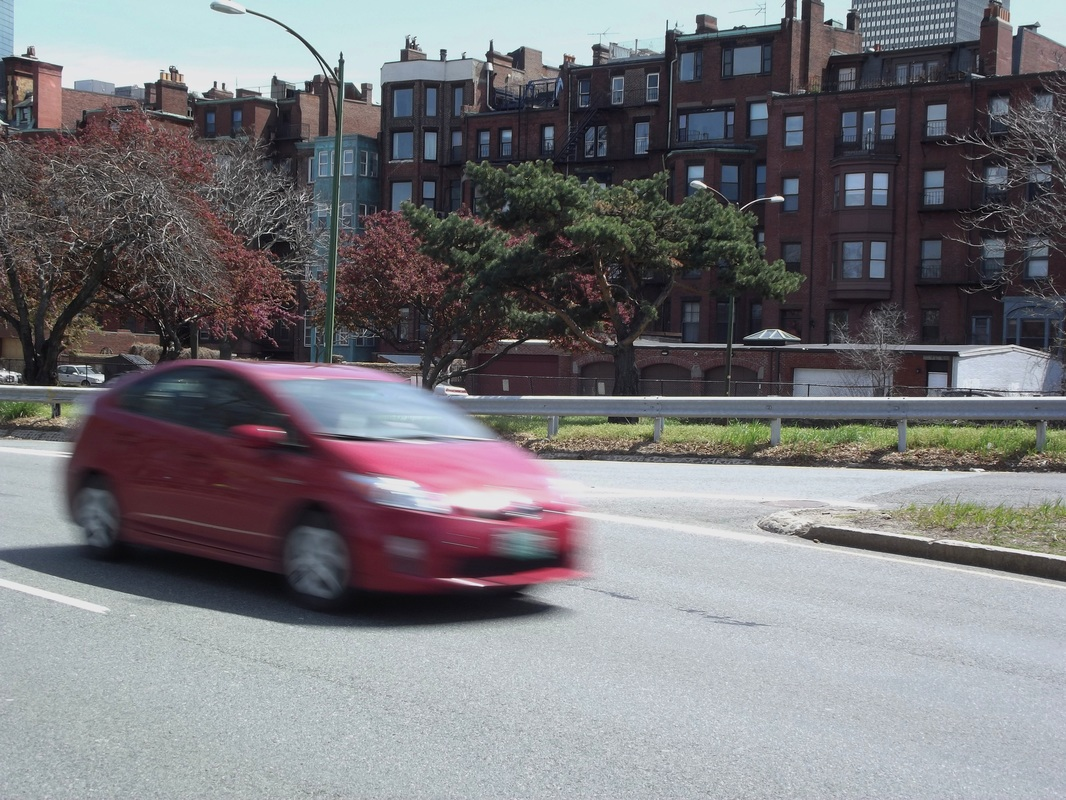
\includegraphics[width=\linewidth]{img/shutter-slow.jpg}
		\caption{Shutter speed van 1/60}
	\end{subfigure}
	\begin{subfigure}[b]{0.4\linewidth}
		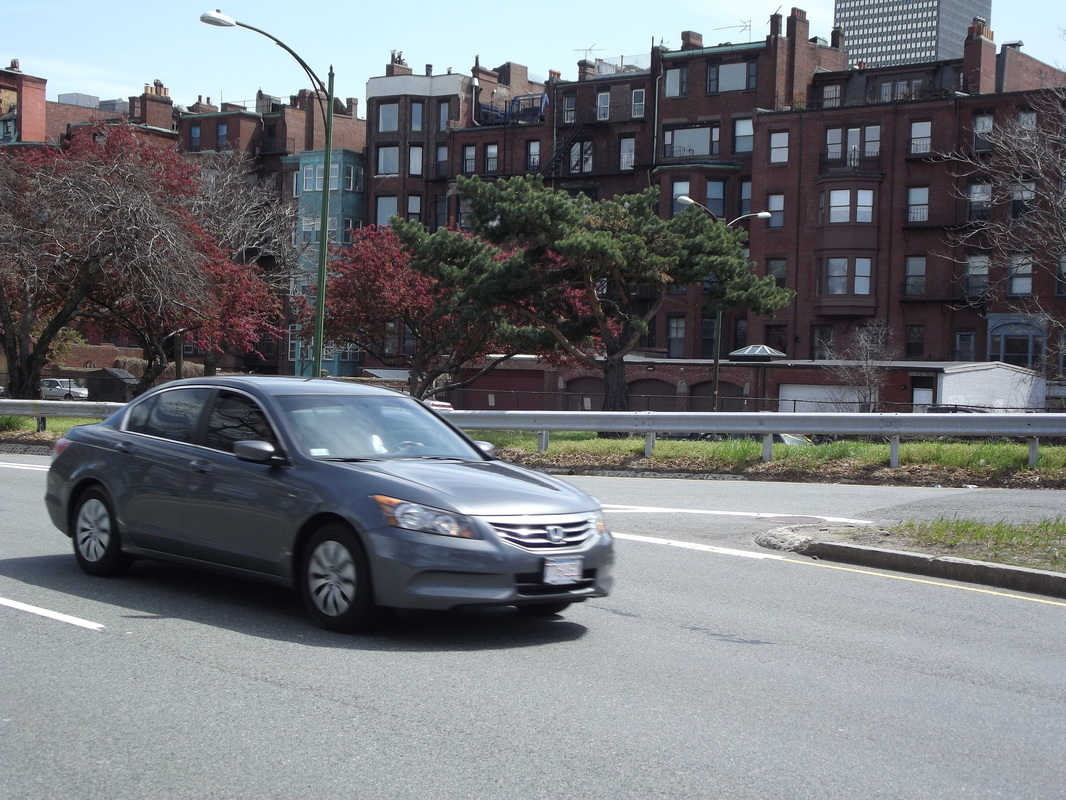
\includegraphics[width=\linewidth]{img/shutter-fast.jpg}
		\caption{Shutter speed van 1/250}
	\end{subfigure}
	\label{fig:ntlpc}
	\caption{Vergelijking van verschillende shutterinstellingen. \autocite{easy2019shutter}}
\end{figure}

Het nadeel van een kleine shutterspeed te nemen is dat er veel minder licht aanwezig is op de foto's, wat de detectie dan weer omlaag brengt. Zo krijg je 's nachts bijna volledig zwarte foto's. Dit kan geremedieerd worden door belichting bij te plaatsen.

\subsection{Belichting}
's Nachts is het moeilijk een degelijke foto van nummerplaten te verkrijgen. Door het weinige licht moet de camera zeer lang zijn shutter openhouden, wat resulteert in een wazige foto.

Men kan de nummerplaat zichtbaar maken door het bijzetten van belichting, maar zelfs dan zal de nummerplaat vaak weinig tot niet zichtbaar zijn. Dit komt doordat de koplampen van een auto zeer fel oplichten in de camera en hierdoor de afbeelding overbelichten. Een algemene oplossing voor deze problemen is het gebruik van een IR-camera. Een IR-camera detecteerd enkel IR-licht en heeft dus geen invloed van de koplampen van wagens. Verder is het voordeel hiervan dat IR-licht niet zichtbaar is voor het menselijk oog, en dus ongestoort snachts en overdag gebruikt kan worden. Een voorbeeld hiervan is te zien in figuur \ref{fig:ir-nacht}, waarbij eerst geen IR-filter wordt gebruikt en daarna wel.

\begin{figure}[h!]
	\centering
	\begin{subfigure}[b]{0.4\linewidth}
		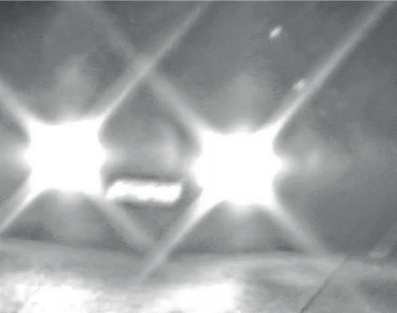
\includegraphics[width=\linewidth]{img/night-time-lpc-bad.png}
		\caption{Slecht geconfigureerde camera.}
	\end{subfigure}
	\begin{subfigure}[b]{0.4\linewidth}
		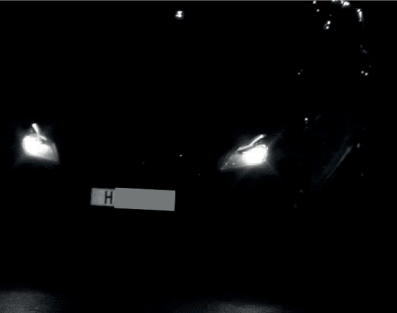
\includegraphics[width=\linewidth]{img/night-time-lpc-good.png}
		\caption{Correct geconfigureerde camera.}
	\end{subfigure}
	\caption{Vergelijking tussen IR-camerainstellingen in de nacht. \autocite{axis2019license}}
	\label{fig:ir-nacht}
\end{figure}

\subsection{Depth of field}
Om scherpe afbeeldingen te verkrijgen moet de depth of field (DOF) van een camera correct ingesteld staan. Deze bepaald in welke range een afbeelding scherp is. Hoe groter de DOF, hoe verder de objecten in focus zijn. Bij afstanden onder de 10m is de DOF aan de kleine kant en moet deze heel nauwkeurig ingesteld worden \autocite{axis2019license}. In vele camera's gebeurt het instellen van de DOF automatisch en moet hier niet echt naar gekeken worden. Een verduidelijking van DOF is te zien in figuur \ref{fig:dof}.

\begin{figure}[h!]
	\centering
	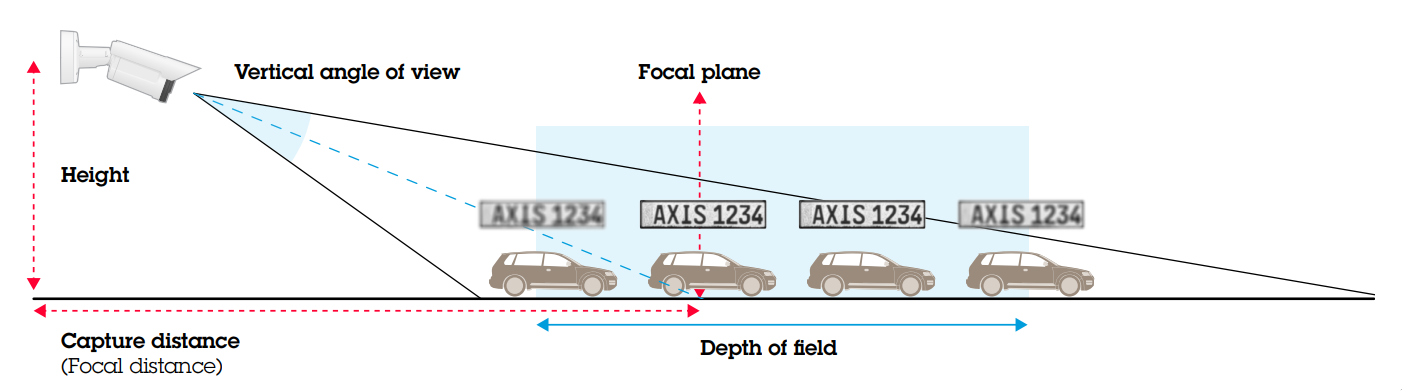
\includegraphics[width=\linewidth]{img/depth-of-field.png}
	\caption{Verduidelijking van depth of field. \autocite{axis2019license}}
	\label{fig:dof}
\end{figure}


\section{Configuratie van OpenALPR}

OpenALPR, de open-source software voor het detecteren van nummerplaten, biedt zelf ook verscheidene instellingen die de accuraatheid van de detectie kan verbeteren. Aangezien de software gebruikt kan worden over heel de wereld zijn en deze nummerplaten heel wat verschillen zijn er meerdere configuraties beschikbaar die specifieker op de regio getraind zijn, maar ook calibratie van de genomen afbeeldingen en patroonmatching zijn beschikbaar.

\subsection{Pattern matching}
\textcite{arrieta2019prototype} en \textcite{buhus2016automatic} concluderen beiden dat openalpr standaard goede resultaten biedt, maar nog hogere resulaten bereikt kunnen worden indien er verduidelijkt wordt welk type nummerplaten er verwacht wordt. Dit houdt factoren in zoals de juiste dataset van het land gebruiken en de volgorde van de kentekenkarakters aanduiden.

Door pattern matching toe te passen kunnen resultaten nog nauwkeuriger zijn. Hierbij wordt een reguliere expressie op alle top N resultaten uitgevoerd en worden de non-matching resultaten verworpen.

Een voorbeeld hiervan is op nummerplaten in Tsjechië, verkregen van \textcite{openalpr2015pattern}
Er wordt nummerplaatdetectie uitgevoerd op afbeelding \ref{patternmatching} met volgende regexpatronen die voorkomen in Tsjechië:
\begin{itemize}
	\item cz \#@\#\#\#\#\#
	\item cz \#@@\#\#\#\#
\end{itemize}

\begin{lstlisting}
[mhill@mhill-linux tmp]$ alpr -c eu -p cz cz_4s50233.jpg -n 40
Config file location provided via default location
plate0: 40 results
- 4S5O233     confidence: 90.947      pattern_match: 0
- 4S5O23      confidence: 87.8683     pattern_match: 0
- 4S5O23      confidence: 85.1644     pattern_match: 0
- 4S5O23S     confidence: 84.5445     pattern_match: 0
- 4S5O23B     confidence: 83.7395     pattern_match: 0
- 4S5O2S3     confidence: 83.3698     pattern_match: 0
- 4S5O23G     confidence: 83.1375     pattern_match: 0
- 4S50233     confidence: 83.0457     pattern_match: 1
- 4S5O2B3     confidence: 82.5635     pattern_match: 0
- 4S5O2       confidence: 82.0857     pattern_match: 0
- 4S5O2G3     confidence: 81.5684     pattern_match: 0
- 4S5O2J3     confidence: 81.0409     pattern_match: 0
- 4S5O2S      confidence: 80.2911     pattern_match: 0
... more results that do not match ...
\end{lstlisting}

\begin{figure}[h!]
	\centering
	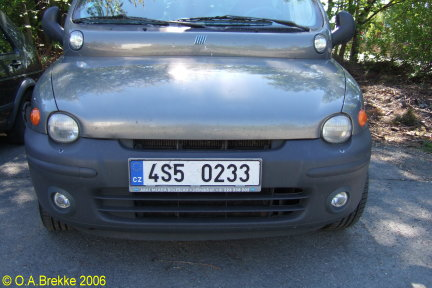
\includegraphics[width=\linewidth]{img/pattern-matching.jpg}
	\caption{Pattern matching van OpenALPR \autocite{openalpr2015pattern}}
	\label{patternmatching}
\end{figure}

Hieruit is te zien dat bij de top 7 resultaten het middelste karakter als de letter O zien i.p.v. het cijfer 0. Door te kijken of de pattern matching succesvol was, zien we dat het achtste resultaat correct is.

\subsection{Calibratie van afbeeldingen}
In vele situaties is het niet mogelijk om de camera frontaal te richten op een nummerplaat. Indien de camera te diagonaal gericht is, zoals in afbeelding \ref{calibration-openalpr}, is het zeer waarschijnlijk dat de accuraatheid van OpenALPR zal zakken. Dit komt omdat OpenALPR getraind is op afbeeldingen die horizontaal gealigneerd zijn met een maximale hoek van 30$^{\circ}$. Gelukkig biedt OpenALPR een eigen tool aan om foto's te kalibreren. Deze is te zien in afbeelding \ref{calibration-openalpr-after}, waar de x- en y-as rotatie en schaal aangepast worden om de afbeelding toch recht te trekken.

\begin{figure}[h!]
	\centering
	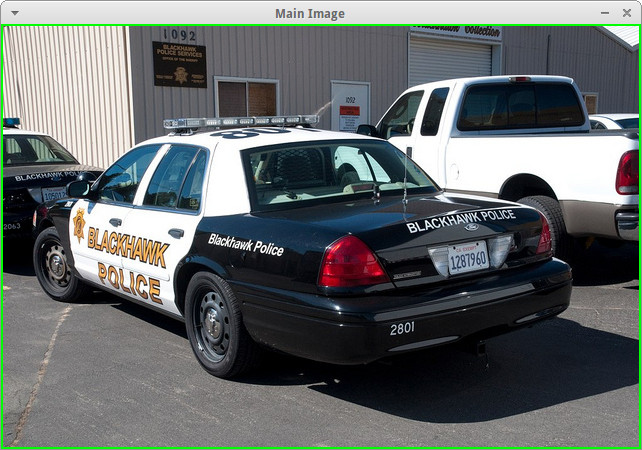
\includegraphics[width=0.7\linewidth]{img/calibration/configuration_calibration_before.jpg}
	\caption{Nummerplaat met een grote invalshoek \autocite{openalpr2015pattern}}
	\label{calibration-openalpr}
\end{figure}

\begin{figure}[h!]
	\centering
	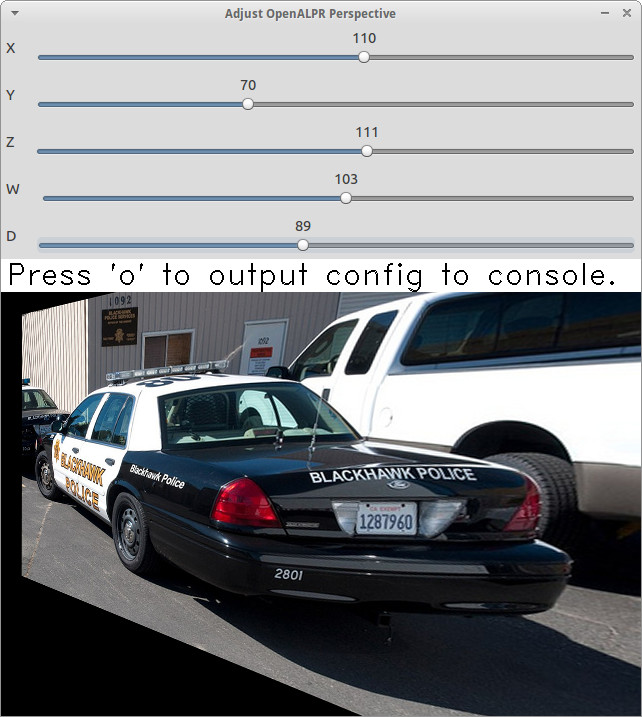
\includegraphics[width=0.7\linewidth]{img/calibration/configuration_calibration_tool.jpg}
	\caption{Gekalibreerde afbeeld adhv. OpenALPR's calibratie tool. \autocite{openalpr2015pattern}}
	\label{calibration-openalpr-after}
\end{figure}

\subsection{Buitenlandse nummerplaten}
OpenALPR heeft verscheidene configuraties voor Europa, Amerika en andere continenten. Door één van deze te selecteren wordt een ander model gekozen dat specifiek voor deze regio is getraind. Bij een keuze van de Europese databank worden er dan ook geen tot weinig fouten verwacht aangezien het model met nummerplaten over heel Europa getraind is.

\subsection{Commerciële upgrades}
OpenALPR biedt ook een commerciële versie aan. Deze zou naar eigen zeggen een hogere nauwkeurigheid bieden in cases waar de Open Source versie slecht presteert \autocite{openalpr2019benchmark}. Er wordt verondersteld dat deze verbeteringen direct zouden vertalen naar het onderzoek zelf en een hogere performantie zal leveren.

De commerciële versie van OpenALPR kost op het moment dat dit onderzoek gepubliceerd is 49 dollar per maand, wat omgerekend 44,1 euro is. Dit onderzoek focust zich op een goedkope implementatie van ANPR, hierdoor wordt de commerciële versie niet overwogen.